% !TeX spellcheck = it_IT 
\documentclass[11pt]{article}
\usepackage[italian]{babel}
\usepackage[T1]{fontenc}
\usepackage[utf8]{inputenc}
\usepackage{graphicx}
\usepackage{todonotes}
\usepackage{listings}
\usepackage{caption}
\usepackage{subcaption}
\usepackage{abbrevs}



\definecolor{dkgreen}{rgb}{0,0.6,0}
\definecolor{gray}{rgb}{0.5,0.5,0.5}
\definecolor{mauve}{rgb}{0.58,0,0.82}

\lstset{
  frame=single,
  captionpos=b,
  language=Java,
  aboveskip=3mm,
  belowskip=3mm,
  showstringspaces=false,
  columns=flexible,
  basicstyle={\small\ttfamily},
  numbers=none,
  numberstyle=\tiny\color{gray},
  keywordstyle=\color{blue},
  commentstyle=\color{dkgreen},
  stringstyle=\color{mauve},
  breaklines=true,
  breakatwhitespace=true,
  tabsize=3
}

\makeatletter
\def\cleardoublepage{
	\clearpage\if@twoside \ifodd\c@page\else
	\hbox{}
	\thispagestyle{empty}
	\newpage
	\if@twocolumn\hbox{}\newpage\fi\fi\fi
}

\makeatother

\setlength{\textwidth}{14cm}
\setlength{\textheight}{21cm}
\setlength{\footskip}{3cm}

\setlength{\hoffset}{0pt}
\setlength{\voffset}{0pt}

\setlength{\oddsidemargin}{1cm}
\setlength{\evensidemargin}{1cm}

\begin{document}
	\title{ROVIS - ROver for VIdeo Streaming\large\\Corso di Fisica dei Sistemi Complessi - Prof. Sandro Rambaldi}

	
	\author{Alessandro Cordella \\Natale Vadalà\\alessandro.cordella@studio.unibo.it\\natale.vadala@studio.unibo.it}\large
	\date{Novembre 2018}
	\maketitle
	\newpage
	\tableofcontents
	\newpage
\section{Introduzione}
L'obiettivo del presente lavoro è stato quello di costruire un robot capace di muoversi su ruote e trasmettere un canale di \textit{streaming video over HTTP}. Il dispositivo ottenuto è controllabile da un'interfaccia web ed è possibile visionare ciò che è posto di fronte al robot tramite una webcam.\\
Nelle seguenti sezioni verranno descritte le fasi di progettazione e realizzazione, i componenti hardware e le tecniche software utilizzate, e verranno presentati eventuali sviluppi futuri.
\section{Progettazione}
La fase di progettazione è stata condotta attraverso l'analisa della specifica e lo studio di progetti open-source precedenti.
\subsection{Specifica}
Progettare e realizzare un robot, controllabile attraverso un'interfaccia Web, dotato di una webcam in modo da poter trasmettere lo streaming video sulla stessa interfaccia.\\
Inoltre, si richiede l'uso di un microcontrollore o di un single-board computer, di componenti low-cost e software open-source.
\subsection{Analisi dei requisiti}
\paragraph{Hardware}
Ciò che serve per realizzare ROVIS:
\begin{itemize}
\item \underline{Microcontrollore / Single-board computer}\\
Si è deciso di utilizzare un RaspberryPi 3 model B\footnote{https://www.raspberrypi.org/products/raspberry-pi-3-model-b/}, che presenta nativamente una scheda di rete wireless, sebbene vada bene un qualsiasi Raspberry dotato di scheda di rete (interna o esterna) e porta USB per la webcam.
\item \underline{Una "carrozzeria" con tutti gli alloggi necessari e 4 motori continui}\\
Per semplicità si è deciso di acquistare un \textit{case}\footnote{https://www.diymore.cc/collections/robot-chassis/products/diymore-4-wheel-robot-chassis-smart-car-with-speed-and-tacho-encoder-for-arduino-raspberry-pi-robot-diy-kits-65x26mm-tire} che comprendesse già i motori fissati, evitando di incorrere in ulteriori future complicazioni con l'asseblaggio e messa in asse delle ruote, del moto, ecc...\\
\item \underline{Una scheda che faccia da driver per i motori}\\
Acquistata su Amazon.it\footnote{http://amzn.eu/d/a9PD82e}, una shield con dei chip L293D\footnote{https://www.robot-italy.com/it/l293d-motor-driver.html} (driver per motori molto comuni), permette di collegare i motori e gestirne la direzione (moto orario/antiorario)  e la velocità, ottebibili grazie allo sfruttamento di alcuni pin GPio d'appoggio per il controllo singolo di ogni motore ai e ponti H per permettere i cambi di direzione. Va alimentato con 5V.
\item \underline{Un Power-bank e un alloggiamento\\ per per shield e motori} \\
Si è deciso di utilizzare un power bank per il RaspberryPi per il semplice motivo che è più comodo, a nostro avviso, servire l'alimentazione da una porta micro USB invece che saldare un ulteriore alloggiamento per batterie sul RaspberryPi (Ma andrebbe comunque un'alimentazione uguale a quella per i motori e la shield, cioè 4* batterie AAA quindi 4.8-5V).

\end{itemize}

\begin{figure}[h!]
				\centering
		\begin{subfigure}[b]{0.6\textwidth}

		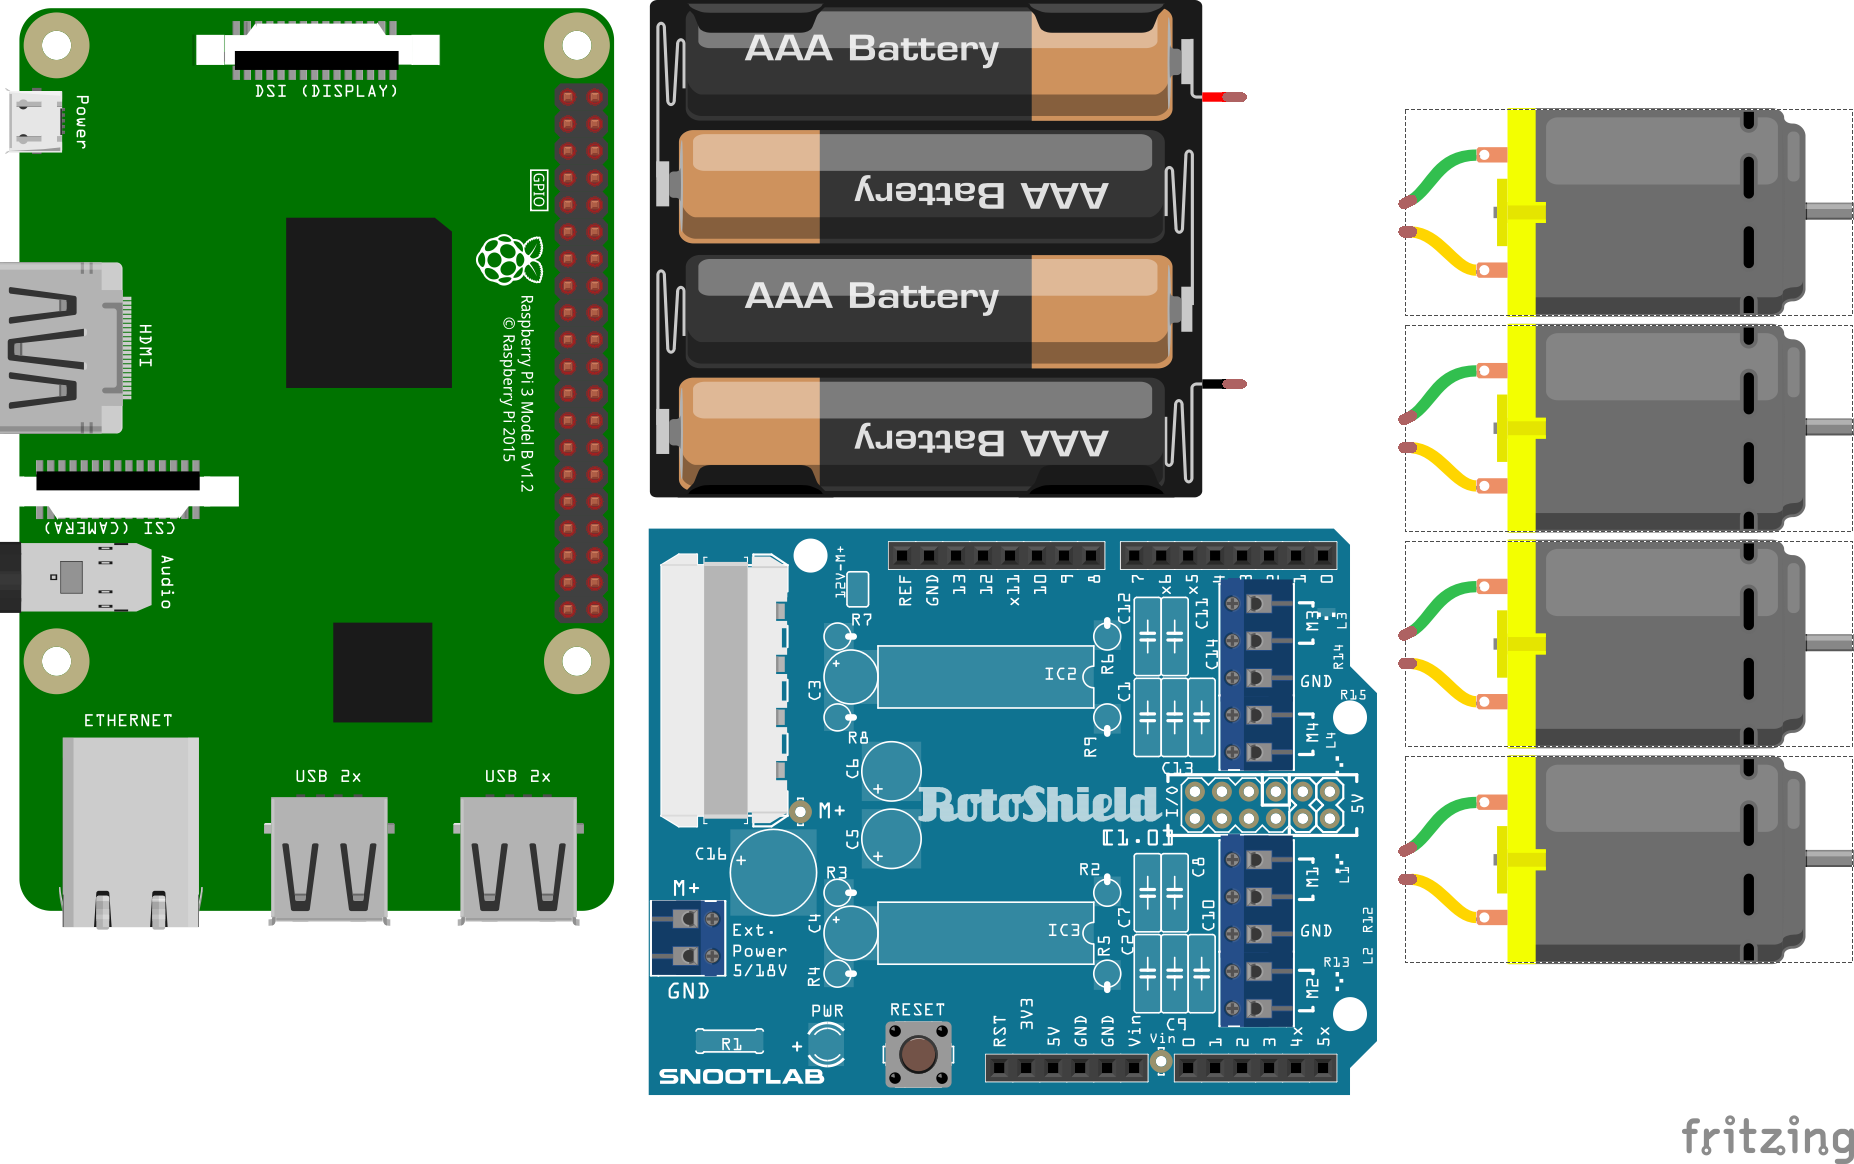
\includegraphics[width=\textwidth]{images/componentsROVIS.png}
		\caption{RaspberryPi, case per batterie, 4 motori continui e L293D drive shield}
		\label{fig:components}
	\end{subfigure}
	%
	\begin{subfigure}[b]{0.4\textwidth}
		
		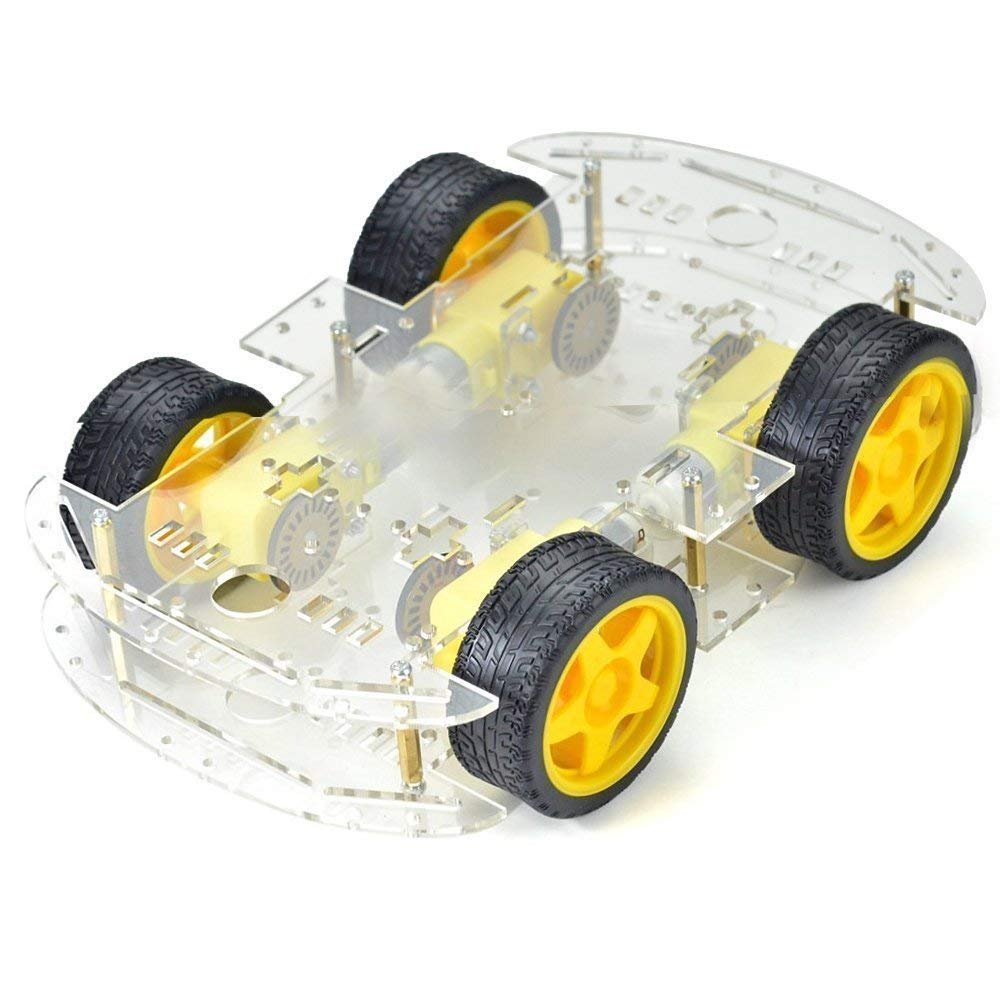
\includegraphics[width=\textwidth]{images/car.jpg}
		\caption{\textit{Case} con motori e ruote}
	\label{fig:car}
	\end{subfigure}
	%
	\begin{subfigure}[b]{0.4\textwidth}
		
		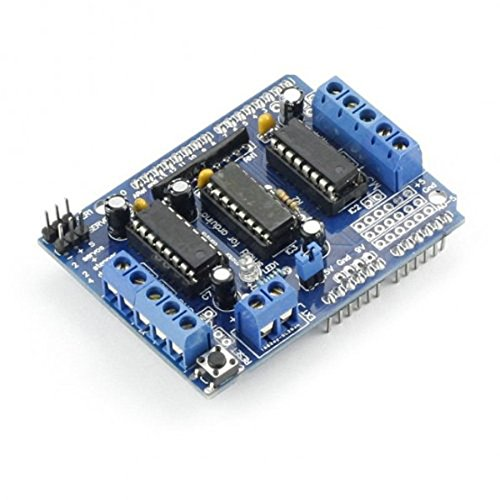
\includegraphics[width=\textwidth]{images/l293d.jpg}
		\caption{L293D drive shield}
	\label{fig:car}
	\end{subfigure}
\end{figure}
\paragraph{Software}

Ciò che serve per realizzare ROVIS:
\begin{itemize}
	\item \underline{Software per acquisizione video e streaming}\\
	Essendo su un sistema operativo Unix, la scelta ricade su ffmpeg\footnote{https://www.ffmpeg.org/}, che permette di codificare/decodificare gli stream video presi in input e restituirne i video in output (online come streaming o offline come file video).
	\item \underline{Piattaforma per orchestrazione dei server}\\
	Per rendere omogeneo e semplice lo sviluppo si è deciso di utilizzare NodeJS\footnote{https://nodejs.org/it/}, che fa al caso nostro (essendo una piattaforma event-driven) e per il semplice motivo che così backend e frontend sono stati scritti entrambi in JavaScript. 
	\item \underline{Stream Server}\\
	Lanciato da NodeJS, di default resta in ascolto sulla porta 8081, è il server che aspetta uno stream MPEG-TS\footnote{https://en.wikipedia.org/wiki/MPEG\_transport\_stream} (streaming video) da parte di ffmpeg, verificandone il \textit{secret} passato come parametro.
	\item \underline{Web Socket Server}\\
		Lanciato da NodeJS, di default resta in ascolto sulla porta 8082, è il server che aspetta una richiesta websocket da parte dello Stream Server.
	\item \underline{HTTP Server}\\
		Lanciato da NodeJS, di default resta in ascolto sulla porta 808, è il componente che serve l'interfaccia web per il controllo di ROVIS, e su cui viene proiettato lo streaming video. Il video è ottenuto dal WebSocket Server e riprodotto in un canvas HTML5.
\end{itemize}
\begin{figure}[h!]
	\centering
	\begin{subfigure}[b]{0.4\textwidth}
		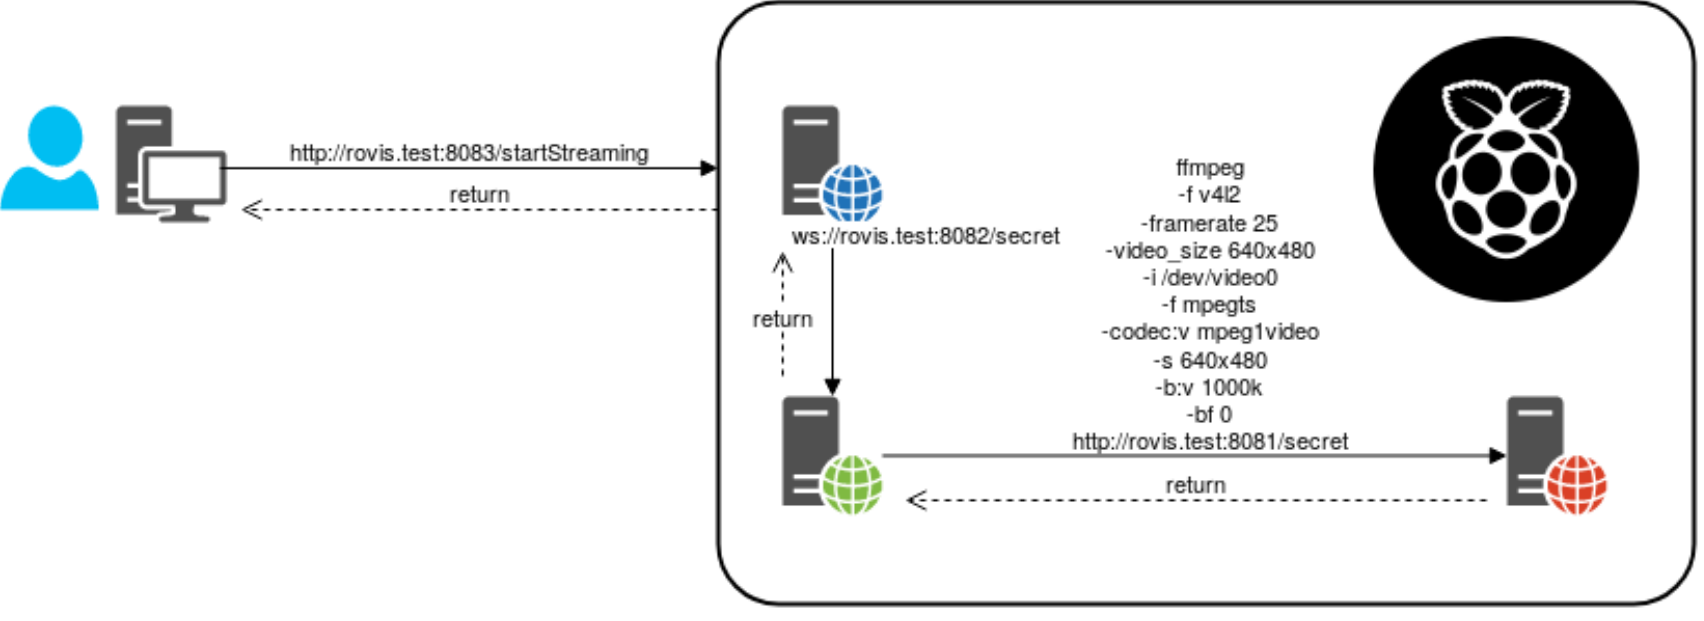
\includegraphics[width=\textwidth]{images/api1.png}
		\caption{Caso d'uso 1: \textbf{\textit{start streaming}}}
		\label{fig:usecase1}
	\end{subfigure}
	%
	\begin{subfigure}[b]{0.4\textwidth}	
		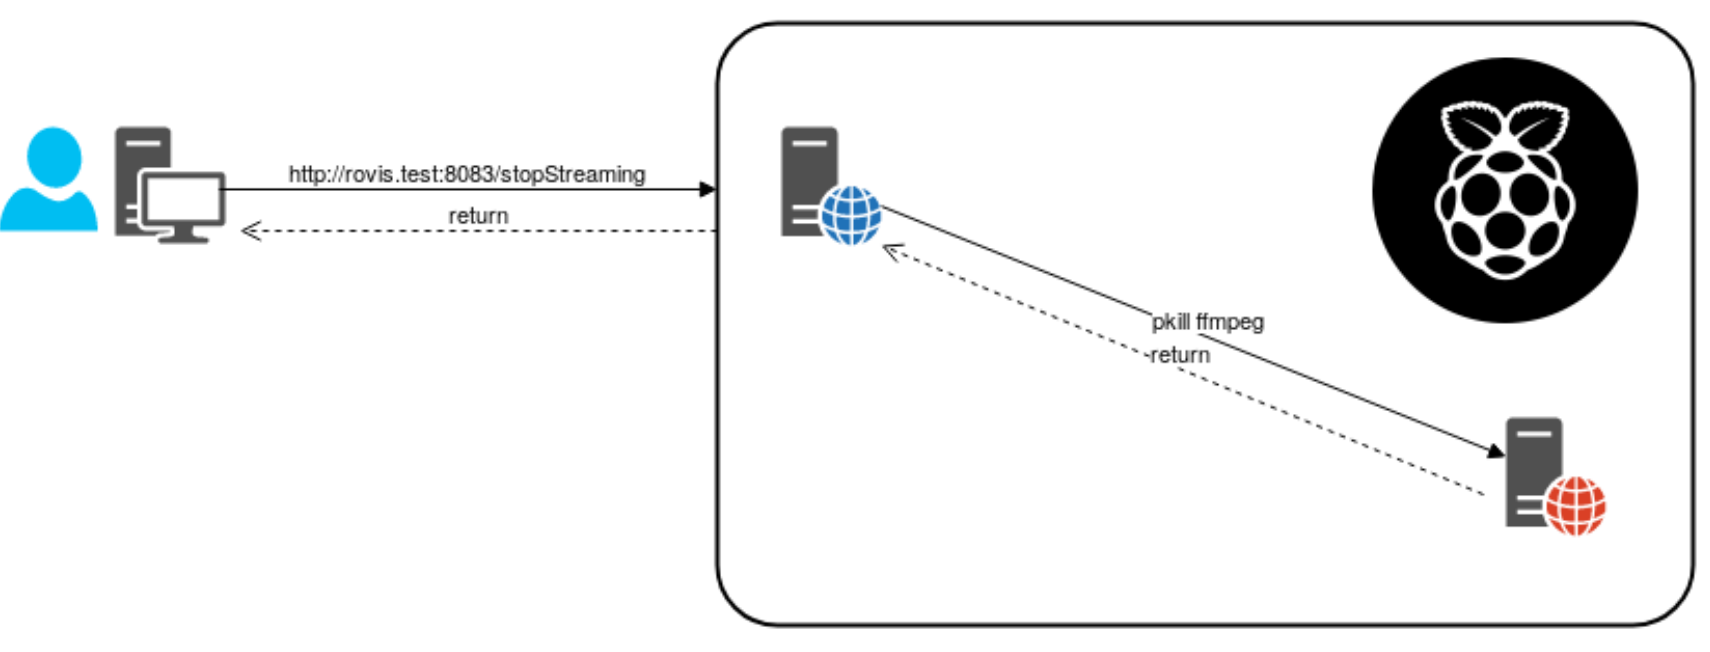
\includegraphics[width=\textwidth]{images/api2.png}
		\caption{Caso d'uso 2: \textbf{\textit{stop streaming}}}
		\label{fig:usecase2}
	\end{subfigure}
	%
	\begin{subfigure}[b]{0.4\textwidth}
		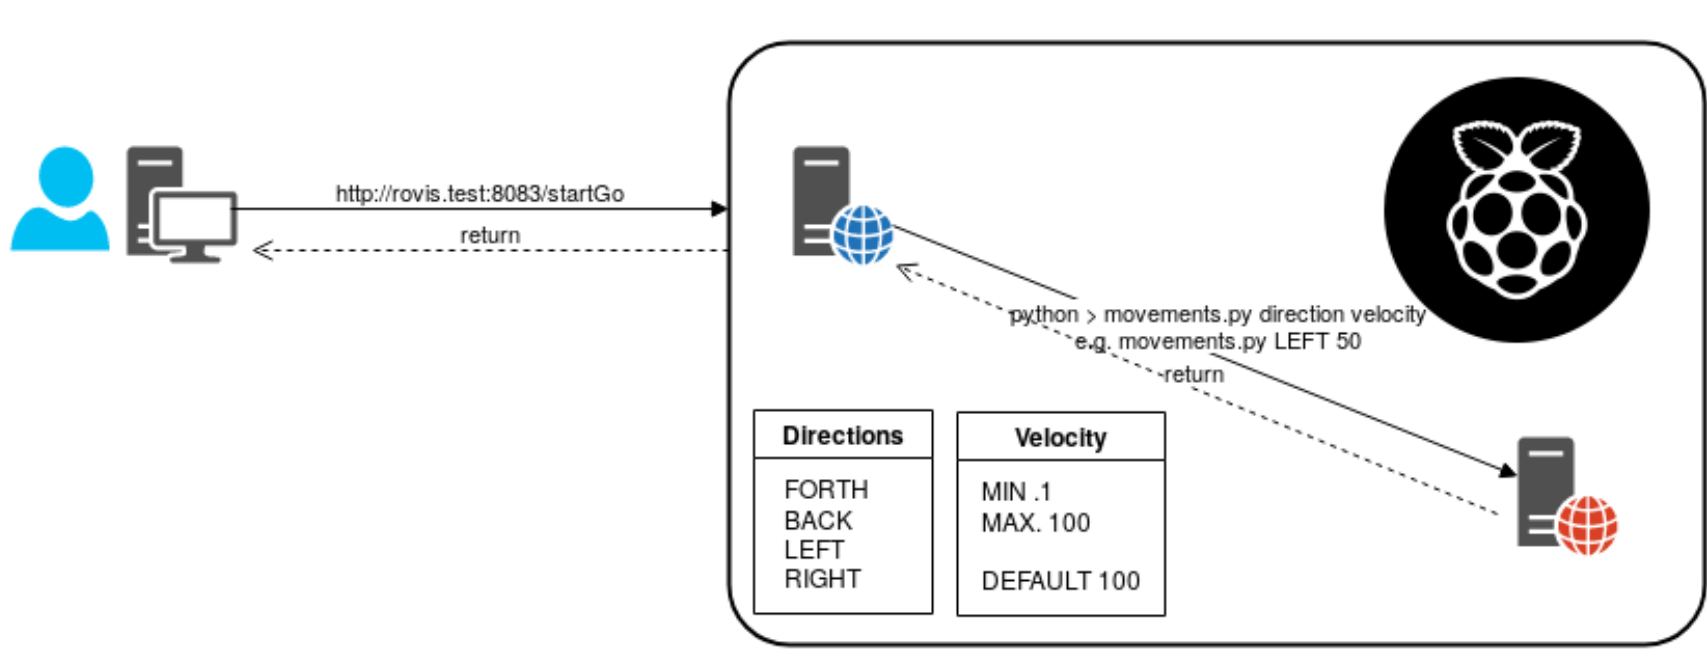
\includegraphics[width=\textwidth]{images/api3.png}
		\caption{Caso d'uso 3: \textbf{\textit{start go}}}
		\label{fig:usecase3}
	\end{subfigure}
	%
	\begin{subfigure}[b]{0.4\textwidth}
		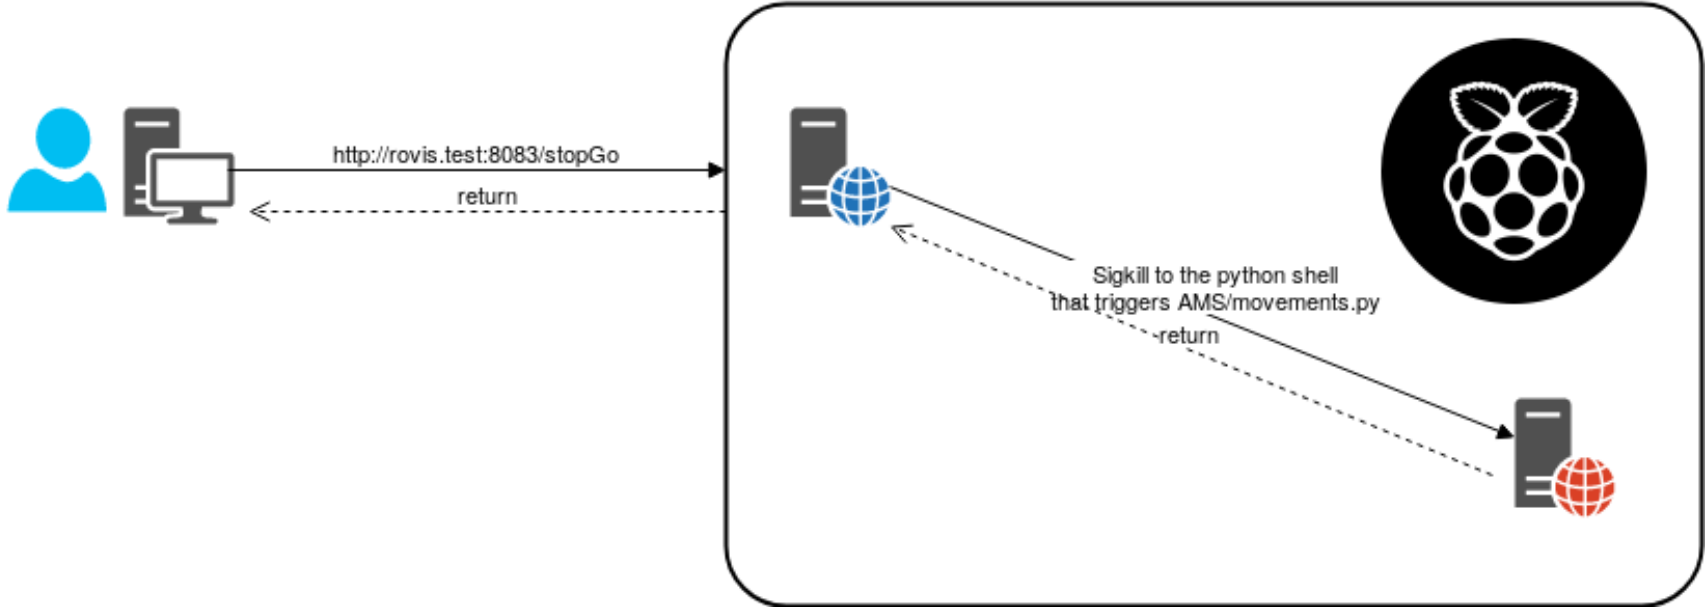
\includegraphics[width=\textwidth]{images/api4.png}
		\caption{Caso d'uso 4: \textbf{\textit{stop go}}}
		\label{fig:usecase4}
	\end{subfigure}
\end{figure}
\section{Realizzazione}
\subsection{Hardware} 
\paragraph{Raspberry e driver}
Lo schema per inizializzare il driver (L293D) in modo che comunichi con il RaspberryPi (poichè la shield è creata per una scheda Arduino-like) e per settare i pin di shift e di controllo è quello trovato nella documentazione della libreria AMSpy.\footnote{https://github.com/lipoja/AMSpi/}\\
Link allo schema.\footnote{https://camo.githubusercontent.com/77d2a42518f0202d0962bdf2431a417d0248f2e5/687474703a2f2f6a616e\\6c69706f76736b792e637a2f776972696e6731322e6a7067}
	\begin{figure}[htp]
		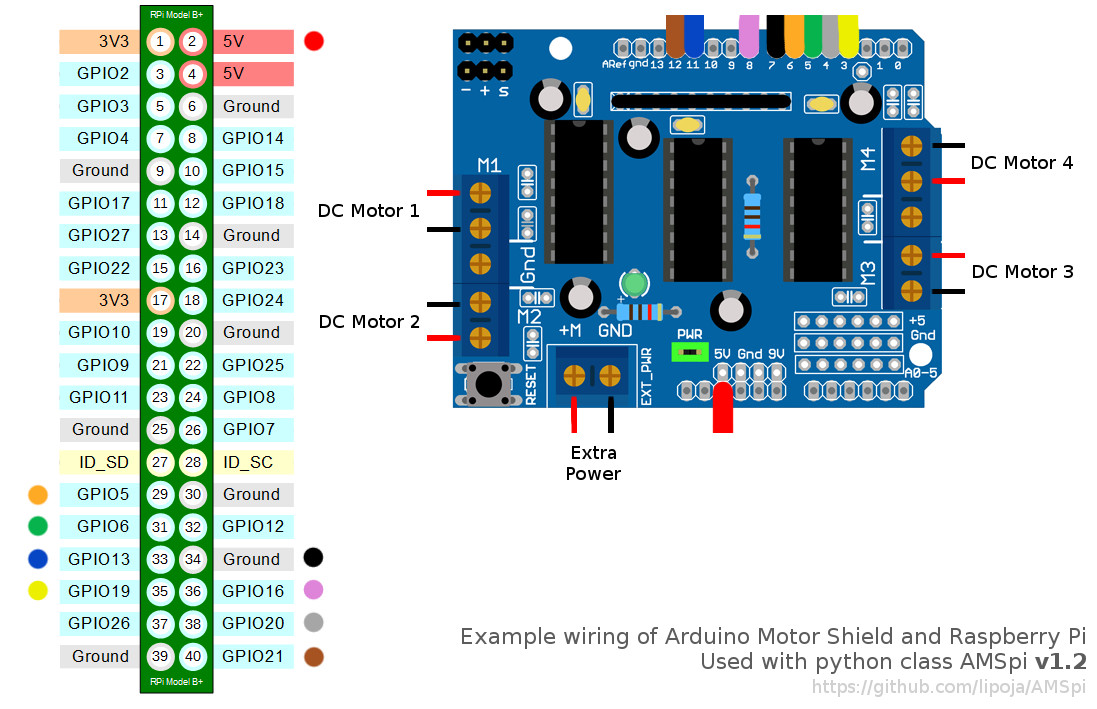
\includegraphics[width=\textwidth]{images/schemaROVIS.jpeg}
		\caption{Schema di connessione tra \textit{driver} e \textit{Raspberry}. }
		\label{fig:schema-driver}
	\end{figure}
\paragraph{Assemblaggio}
\begin{figure}[htp]
	\centering
	\begin{subfigure}[b]{0.5\textwidth}
		\includegraphics[width=\textwidth]{images/rovis-front.png}
		\caption{ROVIS - Vista frontale}
		\label{fig:rovis-front}
	\end{subfigure}
	\\
	%
	\begin{subfigure}[b]{0.5\textwidth}	
		\includegraphics[width=\textwidth]{images/rovis-profile.png}
		\caption{ROVIS - Vista laterale}
		\label{fig:rovis-profile}
	\end{subfigure}
	%
	\begin{subfigure}[b]{0.5\textwidth}
		\includegraphics[width=\textwidth]{images/rovis-top.png}
		\caption{ROVIS - Vista dall'alto}
		\label{fig:rovis-top}
	\end{subfigure}
\end{figure}
\subsection{Software}
Per garantire il controllo del dispositivo tramite un'interfaccia web è stato necessario progettare un server al quale un client può collegarsi. È stato utilizzato il framework JavaScript \textit{NodeJs} per gestire sia la parte client che server dell'applicazione.\\
Inoltre si è dovuto ospitare del Python all'interno del progetto con la libreria AMSpy\footnote{https://github.com/lipoja/AMSpi}, il quale ci ha permesso di controllare la driver shield L293D (Attraverso la libreria Python RPi.GPIO per Raspberry) e ci ha fornito le primitive per inizializzare e settare la shield e interfacciarsi con i motori, cosa che sarebbe stata ben più complessa se avessimo dovuto reimplementare il tutto da zero in JavaScript.
 Nelle seguenti sezioni verrà descritta la struttura gerarchica delle cartelle e le funzionalità presenti nei file al loro interno.
\paragraph{Server side}
I file presenti all'interno della cartella \underline{\textbf{\textit{server /}}} contengono le funzioni per gestire la parte server del sistema, mentre all'interno delle sue sottocartelle sono presenti altri file che verranno descritti in seguito.\\
\subparagraph{.env}
Questo file nascosto, processato da NodeJS, permette di definire le variabili d'ambiente per tutto il progetto. All'interno sono definite le porte di default per i server, il \textit{secret} utilizzato per costruire le richieste, l'indirizzo IP e l'opzione di registrazione. Ovviamente per cambiare \textit{secret}/porte/IP/opzioni basta modificare tale file e rilanciare il progetto.
\begin{lstinputlisting}
	[caption={File .env},basicstyle=\tiny]{codice/env}
\end{lstinputlisting}
\subparagraph{main.js}
Il file \textit{main.js} è il file principale del server. Al suo interno sono presenti le funzioni di inizializzazione del sistema e per la gestione dello streaming video.\\
Qui vengono istanziati i 3 server discussi nel paragrafo 2.2/Software e, inoltre, è definito il percorso da cui servire i files per il frontend.\\
\begin{lstinputlisting}
	[caption={main.js},basicstyle=\tiny]{codice/main}
\end{lstinputlisting}
Per avviare il server è necessario digitare il seguente comando:
\begin{lstinputlisting}
	[caption={Avvio server},basicstyle=\tiny]{codice/startServer}
\end{lstinputlisting}
Una volta lanciato il comando, sarà possibile accedere all'interfaccia web digitando l'indirizzo IP del Raspberry seguito dalla porta su cui gira l'HTML server (default 8083).
\begin{lstinputlisting}[caption={Esempio indirizzo server},basicstyle=\tiny]{codice/indirizzo}
\end{lstinputlisting}
\subparagraph{routes.js}
Questo file è quello che definisce le API, cioè gestisce la comunicazione client-server, associando ad ogni interazione del client sulla pagina web una specifica azione del server. Gestisce quindi le funzioni che regolano la webcam e il movimento. In particolare viene utilizzata la libreria di NodeJS \textit{python-shell}\footnote{https://www.npmjs.com/package/python-shell} per eseguire uno script Python prodotto da noi (\textit{movements.py}) per la gestione dei motori.
\begin{lstinputlisting}[caption={routes.js},basicstyle=\tiny]{codice/routes}
\end{lstinputlisting}
\subparagraph{\underline{AMSpi/}}
\textit{AMSpi} è la libreria Python utilizzata per controllare i motori. 
\subparagraph{AMSpi/movements.py}
Script scritto da noi che sfrutta la libreria. Inizialmente setta i pin GPIO d'appoggio per i ponti H e i 4 pin per controllare ogni motore. In seguito triggera le azioni di \textit{start} e \textit{stop} dei motori, in base alla direzione e alla velocità passata come input.
\begin{lstinputlisting}[caption={AMSpy/movements.py},basicstyle=\tiny]{codice/movements}
\end{lstinputlisting}
\paragraph{Client side}
I file presenti all'interno della cartella \underline{\textbf{\textit{public/}}} sono quelli che gestiscono la parte client dell'applicazione.\\
\subparagraph{index.html} 
\todo{immagine}
È il file contenente la struttura HTML del sito web.
\subparagraph{\underline{css/}}
All'interno di questa cartella sono presenti i file che regolano lo stile della pagina.
\subparagraph{\underline{js/}}
In questa cartella sono contenuti i file che regolano le interazioni dell'utente con la pagina e comunicano al server le azioni intraprese da esso.
\subparagraph{js/arrow.js}
Binding fra eventi sulla pagina web (click con il mouse/ click su tastiera) e azioni (richieste HTTP Get) dal browser dell'utente al server.
\begin{lstinputlisting}[caption={js/arrow.js},basicstyle=\tiny]{codice/arrow}
\end{lstinputlisting}
\subparagraph{js/canvas.js}
Fetching dell'elemento \textit{video-canvas} sull'HTML, e dell'indirizzo del web socket server, per istanziare un oggetto di tipo JSMPEG Player (Il componente che riproduce il video su browser).
\subparagraph{js/jsmpeg.min.js}
Libreria JavaScript importata staticamente\footnote{https://github.com/phoboslab/jsmpeg}, offre la possibilità di istanziare e utilizzare Video player, con relativi decoder (MPEG-TS, MPEG-1)  e renderers (WebGL, Canvas2D).

\section{Conclusioni e Sviluppi futuri}
L'obiettivo del presente lavoro è stato quello di costruire un robot capace di muoversi su ruote e trasmettere un canale di \textit{streaming video over HTTP}. Il robot ROVIS è stato realizzato coerentemente alla specifica.\\
Il dispositivo ROVIS potrebbero essere ulteriormente migliorato implementando le seguenti funzionalità:
\begin{itemize}
	\item Installazione di un modulo con sensori ad ultrasuoni con il fine di evitare lo scontro di ROVIS con ostacoli;
	\item Creazione un'applicazione Android per gestire il dispositivo;
	\item Configurazione del sistema al fine di consentire un accesso alla pagina di gestione da remoto.
\end{itemize}

%\newpage	
%\bibliographystyle{abbrv}
%\bibliography{Bib}
\end{document}